\input{header.tex}
\input{newcommands.tex}


\title{Geometrische Figuren mit \TikZ zeichnen}
\author{Fortbildungsmaterial für MINT-Lehrkräfte}
\date{\today}
\pagestyle{plain}
\setlength{\parskip}{1.5em} % Abstand zwischen Absätzen (Handreichungen)


\begin{document}

\maketitle

Dreiecke, Kreise, Konstruktionen und Körper gehören in jeder Klassenstufe zum Geometrieunterricht. Diese Handreichung gibt feste Vorlagen vor, die alle denselben Gestaltungsregeln folgen. So sehen Skizzen auf allen Arbeitsblättern gleich aus und lassen sich schnell an neue Maße anpassen.



%%%%  KAPITEL 1  %%%%
\section{Gestaltungsregeln für geometrische Figuren}

Alle Figuren folgen denselben Regeln, damit Arbeitsblätter einheitlich aussehen: Die Hauptfigur wird mit \texttt{blue, very thick} gezeichnet, Maße, Winkel und Hervorhebungen mit \texttt{red, thick}, Hilfs- und verdeckte Linien gestrichelt, Konstruktionslinien \texttt{gray, thin}, Flächen mit \texttt{gray, opacity=0.5}. Eckpunkte werden als \texttt{\textbackslash coordinate} definiert und erst danach verwendet. Die benötigten Bibliotheken (\texttt{calc}, \texttt{angles}, \texttt{quotes}) sind in der universalen \texttt{header.tex} geladen.



%%%%  KAPITEL 2  %%%%
\section{Dreiecke}


%%%%  UNTERKAPITEL 2.1  %%%%
\subsection{Dreieck mit Ecken, Seiten und Winkeln}

Winkel werden mit der \texttt{angles}-Bibliothek als \texttt{pic} gezeichnet. \texttt{angle=B--A--C} misst gegen den Uhrzeigersinn von $AB$ nach $AC$. Seiten werden mit \texttt{calc} in der Mitte beschriftet:

\begin{lstlisting}[style=latex]
\begin{tikzpicture}
	% Eckpunkte
	\coordinate (A) at (0,0);
	\coordinate (B) at (5,0);
	\coordinate (C) at (1.5,3);
	% Winkel (Bibliotheken angles und quotes), zuerst, damit die Seiten darüber liegen
	\pic[draw=red, thick, "$\alpha$", angle radius=0.6cm, angle eccentricity=1.6] {angle=B--A--C};
	\pic[draw=red, thick, "$\beta$", angle radius=0.6cm, angle eccentricity=1.6] {angle=C--B--A};
	\pic[draw=red, thick, "$\gamma$", angle radius=0.6cm, angle eccentricity=1.6] {angle=A--C--B};
	% Dreieck
	\draw[blue, very thick] (A) -- (B) -- (C) -- cycle;
	% Beschriftung der Ecken
	\node[below left] at (A) {$A$};
	\node[below right] at (B) {$B$};
	\node[above] at (C) {$C$};
	% Seiten liegen der gleichnamigen Ecke gegenüber
	\node[below] at ($(A)!0.5!(B)$) {$c$};
	\node[above right] at ($(B)!0.5!(C)$) {$a$};
	\node[above left] at ($(A)!0.5!(C)$) {$b$};
\end{tikzpicture}
\end{lstlisting}

\begin{ausgabe}
\centering
\begin{tikzpicture}
	% Eckpunkte
	\coordinate (A) at (0,0);
	\coordinate (B) at (5,0);
	\coordinate (C) at (1.5,3);
	% Winkel (Bibliotheken angles und quotes), zuerst, damit die Seiten darüber liegen
	\pic[draw=red, thick, "$\alpha$", angle radius=0.6cm, angle eccentricity=1.6] {angle=B--A--C};
	\pic[draw=red, thick, "$\beta$", angle radius=0.6cm, angle eccentricity=1.6] {angle=C--B--A};
	\pic[draw=red, thick, "$\gamma$", angle radius=0.6cm, angle eccentricity=1.6] {angle=A--C--B};
	% Dreieck
	\draw[blue, very thick] (A) -- (B) -- (C) -- cycle;
	% Beschriftung der Ecken
	\node[below left] at (A) {$A$};
	\node[below right] at (B) {$B$};
	\node[above] at (C) {$C$};
	% Seiten liegen der gleichnamigen Ecke gegenüber
	\node[below] at ($(A)!0.5!(B)$) {$c$};
	\node[above right] at ($(B)!0.5!(C)$) {$a$};
	\node[above left] at ($(A)!0.5!(C)$) {$b$};
\end{tikzpicture}
\end{ausgabe}


%%%%  UNTERKAPITEL 2.2  %%%%
\subsection{Rechtwinkliges Dreieck}

Der rechte Winkel bekommt einen Punkt im Winkelbogen:

\begin{lstlisting}[style=latex]
\begin{tikzpicture}
	\coordinate (A) at (0,0);
	\coordinate (B) at (4,0);
	\coordinate (C) at (0,3);
	% rechter Winkel als Viertelkreis mit Punkt
	\pic[draw=red, thick, angle radius=0.5cm] {angle=B--A--C};
	\node[red] at (0.2,0.2) {$\cdot$};
	\draw[blue, very thick] (A) -- (B) -- (C) -- cycle;
	\node[below left] at (A) {$A$};
	\node[below right] at (B) {$B$};
	\node[above left] at (C) {$C$};
	\node[below] at ($(A)!0.5!(B)$) {Kathete $c$};
	\node[left] at ($(A)!0.5!(C)$) {Kathete $b$};
	\node[above right] at ($(B)!0.5!(C)$) {Hypotenuse $a$};
\end{tikzpicture}
\end{lstlisting}

\begin{ausgabe}
\centering
\begin{tikzpicture}
	\coordinate (A) at (0,0);
	\coordinate (B) at (4,0);
	\coordinate (C) at (0,3);
	% rechter Winkel als Viertelkreis mit Punkt
	\pic[draw=red, thick, angle radius=0.5cm] {angle=B--A--C};
	\node[red] at (0.2,0.2) {$\cdot$};
	\draw[blue, very thick] (A) -- (B) -- (C) -- cycle;
	\node[below left] at (A) {$A$};
	\node[below right] at (B) {$B$};
	\node[above left] at (C) {$C$};
	\node[below] at ($(A)!0.5!(B)$) {Kathete $c$};
	\node[left] at ($(A)!0.5!(C)$) {Kathete $b$};
	\node[above right] at ($(B)!0.5!(C)$) {Hypotenuse $a$};
\end{tikzpicture}
\end{ausgabe}


%%%%  UNTERKAPITEL 2.3  %%%%
\subsection{Höhe mit rechtem Winkel}

Für den rechten Winkel gibt es das Symbol \texttt{right angle}:

\begin{lstlisting}[style=latex]
\begin{tikzpicture}
	\coordinate (A) at (0,0);
	\coordinate (B) at (5,0);
	\coordinate (C) at (1.5,3);
	\coordinate (H) at (1.5,0);   % Fußpunkt der Höhe
	\draw[blue, very thick] (A) -- (B) -- (C) -- cycle;
	% Höhe gestrichelt mit rechtem Winkel
	\draw[blue, dashed] (C) -- (H);
	\pic[draw=red, thick, angle radius=0.35cm] {right angle=B--H--C};
	\node[right] at ($(C)!0.5!(H)$) {$h_c$};
	\node[below left] at (A) {$A$};
	\node[below right] at (B) {$B$};
	\node[above] at (C) {$C$};
	\node[below] at (H) {$H$};
\end{tikzpicture}
\end{lstlisting}

\begin{ausgabe}
\centering
\begin{tikzpicture}
	\coordinate (A) at (0,0);
	\coordinate (B) at (5,0);
	\coordinate (C) at (1.5,3);
	\coordinate (H) at (1.5,0);   % Fußpunkt der Höhe
	\draw[blue, very thick] (A) -- (B) -- (C) -- cycle;
	% Höhe gestrichelt mit rechtem Winkel
	\draw[blue, dashed] (C) -- (H);
	\pic[draw=red, thick, angle radius=0.35cm] {right angle=B--H--C};
	\node[right] at ($(C)!0.5!(H)$) {$h_c$};
	\node[below left] at (A) {$A$};
	\node[below right] at (B) {$B$};
	\node[above] at (C) {$C$};
	\node[below] at (H) {$H$};
\end{tikzpicture}
\end{ausgabe}



%%%%  KAPITEL 3  %%%%
\section{Maße, Kreise und Vierecke}


%%%%  UNTERKAPITEL 3.1  %%%%
\subsection{Maßlinien und Teilflächen}

Maßlinien liegen mit etwas Abstand neben der Figur und haben Begrenzungsstriche: \texttt{|<->|}. Einheiten mit \texttt{\textbackslash unit}:

\begin{lstlisting}[style=latex]
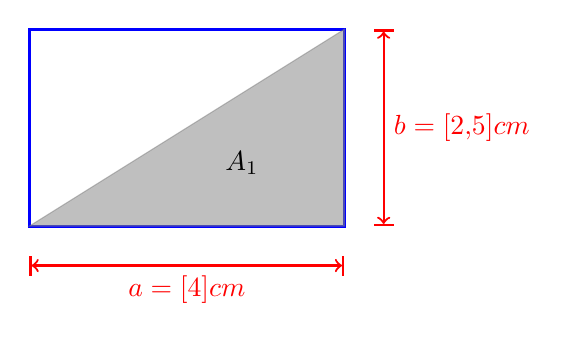
\begin{tikzpicture}
	% Hauptfigur
	\draw[blue, very thick] (0,0) rectangle (4,2.5);
	% Maßlinien mit Abstand zur Figur
	\draw[|<->|, red, thick] (0,-0.5) -- node[below] {$a = \unit[4]{cm}$} (4,-0.5);
	\draw[|<->|, red, thick] (4.5,0) -- node[right] {$b = \unit[2{,}5]{cm}$} (4.5,2.5);
	% gefärbte Fläche
	\filldraw[gray, opacity=0.5] (0,0) -- (4,0) -- (4,2.5) -- cycle;
	\node at (2.7,0.8) {$A_1$};
\end{tikzpicture}
\end{lstlisting}

\begin{ausgabe}
\centering
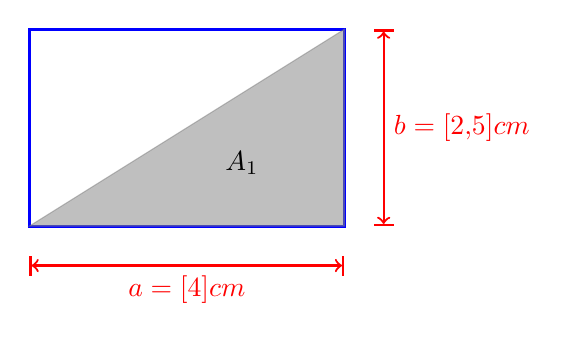
\begin{tikzpicture}
	% Hauptfigur
	\draw[blue, very thick] (0,0) rectangle (4,2.5);
	% Maßlinien mit Abstand zur Figur
	\draw[|<->|, red, thick] (0,-0.5) -- node[below] {$a = \unit[4]{cm}$} (4,-0.5);
	\draw[|<->|, red, thick] (4.5,0) -- node[right] {$b = \unit[2{,}5]{cm}$} (4.5,2.5);
	% gefärbte Fläche
	\filldraw[gray, opacity=0.5] (0,0) -- (4,0) -- (4,2.5) -- cycle;
	\node at (2.7,0.8) {$A_1$};
\end{tikzpicture}
\end{ausgabe}


%%%%  UNTERKAPITEL 3.2  %%%%
\subsection{Kreis, Radius, Durchmesser und Sektor}

\begin{lstlisting}[style=latex]
\begin{tikzpicture}
	\coordinate (M) at (0,0);
	\coordinate (A) at (0:2);
	\coordinate (B) at (60:2);
	% Kreissektor mit Mittelpunktswinkel 60°
	\filldraw[gray, opacity=0.5] (M) -- (0:2) arc[start angle=0, end angle=60, radius=2] -- cycle;
	\draw[blue, very thick] (M) circle (2);
	% Radius und Durchmesser
	\draw[red, thick] (M) -- node[below] {$r$} (0:2);
	\draw[red, thick, dashed] (150:2) -- node[above, sloped] {$d$} (330:2);
	% Winkel im Sektor
	\pic[draw=red, thick, "$60^\circ$", angle radius=0.7cm, angle eccentricity=1.6] {angle=A--M--B};
	\node[punkt, label=below left:$M$] at (M) {};
\end{tikzpicture}
\end{lstlisting}

\begin{ausgabe}
\centering
\begin{tikzpicture}
	\coordinate (M) at (0,0);
	\coordinate (A) at (0:2);
	\coordinate (B) at (60:2);
	% Kreissektor mit Mittelpunktswinkel 60°
	\filldraw[gray, opacity=0.5] (M) -- (0:2) arc[start angle=0, end angle=60, radius=2] -- cycle;
	\draw[blue, very thick] (M) circle (2);
	% Radius und Durchmesser
	\draw[red, thick] (M) -- node[below] {$r$} (0:2);
	\draw[red, thick, dashed] (150:2) -- node[above, sloped] {$d$} (330:2);
	% Winkel im Sektor
	\pic[draw=red, thick, "$60^\circ$", angle radius=0.7cm, angle eccentricity=1.6] {angle=A--M--B};
	\node[punkt, label=below left:$M$] at (M) {};
\end{tikzpicture}
\end{ausgabe}


%%%%  UNTERKAPITEL 3.3  %%%%
\subsection{Parallelogramm und Trapez}

Mit \texttt{scope} und \texttt{xshift} stehen mehrere Figuren nebeneinander in einem Bild:

\begin{lstlisting}[style=latex]
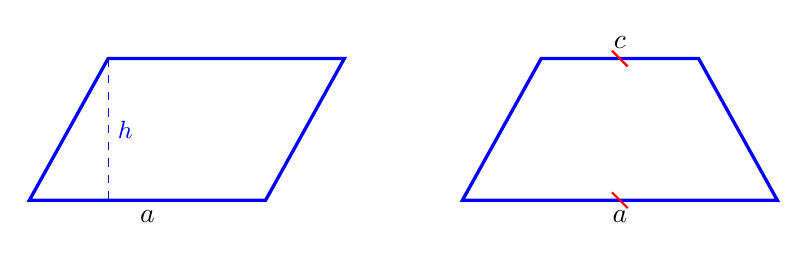
\begin{tikzpicture}
	% Parallelogramm
	\draw[blue, very thick] (0,0) -- (3,0) -- (4,1.8) -- (1,1.8) -- cycle;
	\draw[blue, dashed] (1,1.8) -- node[right] {\small $h$} (1,0);
	\node[below] at (1.5,0) {$a$};
	% Trapez
	\begin{scope}[xshift=5.5cm]
		\draw[blue, very thick] (0,0) -- (4,0) -- (3,1.8) -- (1,1.8) -- cycle;
		\node[below] at (2,0) {$a$};
		\node[above] at (2,1.8) {$c$};
		% parallele Seiten markieren
		\draw[red, thick] (1.9,0.1) -- (2.1,-0.1) (1.9,1.9) -- (2.1,1.7);
	\end{scope}
\end{tikzpicture}
\end{lstlisting}

\begin{ausgabe}
\centering
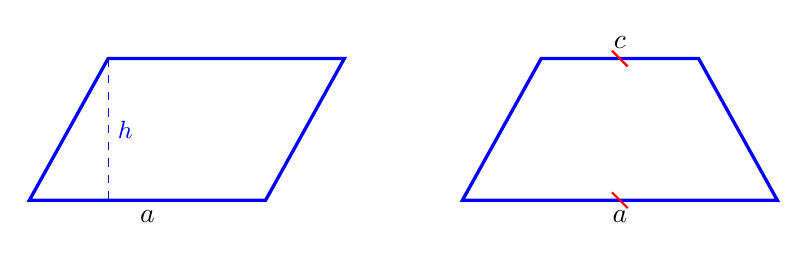
\begin{tikzpicture}
	% Parallelogramm
	\draw[blue, very thick] (0,0) -- (3,0) -- (4,1.8) -- (1,1.8) -- cycle;
	\draw[blue, dashed] (1,1.8) -- node[right] {\small $h$} (1,0);
	\node[below] at (1.5,0) {$a$};
	% Trapez
	\begin{scope}[xshift=5.5cm]
		\draw[blue, very thick] (0,0) -- (4,0) -- (3,1.8) -- (1,1.8) -- cycle;
		\node[below] at (2,0) {$a$};
		\node[above] at (2,1.8) {$c$};
		% parallele Seiten markieren
		\draw[red, thick] (1.9,0.1) -- (2.1,-0.1) (1.9,1.9) -- (2.1,1.7);
	\end{scope}
\end{tikzpicture}
\end{ausgabe}



%%%%  KAPITEL 4  %%%%
\section{Konstruktionen}


%%%%  UNTERKAPITEL 4.1  %%%%
\subsection{Mittelsenkrechte mit Zirkelbögen}

Zirkelbögen sind Konstruktionslinien in Grau; das Ergebnis ist blau. Die Bögen werden mit \texttt{++(Winkel:Radius) arc} vom Mittelpunkt aus angesetzt:

\begin{lstlisting}[style=latex]
\begin{tikzpicture}
	\coordinate (A) at (0,0);
	\coordinate (B) at (4,0);
	% Zirkelbögen um A und B mit gleichem Radius (Konstruktionslinien grau)
	\draw[gray, thin] (A) ++(25:2.8) arc[start angle=25, end angle=65, radius=2.8];
	\draw[gray, thin] (A) ++(-65:2.8) arc[start angle=-65, end angle=-25, radius=2.8];
	\draw[gray, thin] (B) ++(115:2.8) arc[start angle=115, end angle=155, radius=2.8];
	\draw[gray, thin] (B) ++(205:2.8) arc[start angle=205, end angle=245, radius=2.8];
	% Ergebnis: Mittelsenkrechte durch die Schnittpunkte der Bögen
	\draw[blue, very thick] (2,-2.6) -- (2,2.6) node[above] {$m_{AB}$};
	\draw[blue, very thick] (A) -- (B);
	\node[punkt, label=below left:$A$] at (A) {};
	\node[punkt, label=below right:$B$] at (B) {};
	\node[punkt, label=below right:$M$] at (2,0) {};
\end{tikzpicture}
\end{lstlisting}

\begin{ausgabe}
\centering
\begin{tikzpicture}
	\coordinate (A) at (0,0);
	\coordinate (B) at (4,0);
	% Zirkelbögen um A und B mit gleichem Radius (Konstruktionslinien grau)
	\draw[gray, thin] (A) ++(25:2.8) arc[start angle=25, end angle=65, radius=2.8];
	\draw[gray, thin] (A) ++(-65:2.8) arc[start angle=-65, end angle=-25, radius=2.8];
	\draw[gray, thin] (B) ++(115:2.8) arc[start angle=115, end angle=155, radius=2.8];
	\draw[gray, thin] (B) ++(205:2.8) arc[start angle=205, end angle=245, radius=2.8];
	% Ergebnis: Mittelsenkrechte durch die Schnittpunkte der Bögen
	\draw[blue, very thick] (2,-2.6) -- (2,2.6) node[above] {$m_{AB}$};
	\draw[blue, very thick] (A) -- (B);
	\node[punkt, label=below left:$A$] at (A) {};
	\node[punkt, label=below right:$B$] at (B) {};
	\node[punkt, label=below right:$M$] at (2,0) {};
\end{tikzpicture}
\end{ausgabe}



%%%%  KAPITEL 5  %%%%
\section{Körper im Schrägbild}

Körper werden in Kavalierperspektive gezeichnet: Kanten in die Tiefe unter $45^\circ$ und halb so lang. Verdeckte Kanten sind gestrichelt und werden zuerst gezeichnet.


%%%%  UNTERKAPITEL 5.1  %%%%
\subsection{Quader}

\begin{lstlisting}[style=latex]
% Schrägbild in Kavalierperspektive: Tiefe unter 45° und halb so lang
\begin{tikzpicture}
	\def\b{4} \def\h{2} \def\t{3}
	\coordinate (A) at (0,0);   \coordinate (B) at (\b,0);
	\coordinate (C) at (\b,\h); \coordinate (D) at (0,\h);
	\coordinate (E) at ($(A)+(45:\t*0.5)$); \coordinate (F) at ($(B)+(45:\t*0.5)$);
	\coordinate (G) at ($(C)+(45:\t*0.5)$); \coordinate (H) at ($(D)+(45:\t*0.5)$);
	% verdeckte Kanten gestrichelt
	\draw[blue, dashed] (A) -- (E) -- (F) (E) -- (H);
	% sichtbare Kanten
	\draw[blue, very thick] (A) -- (B) -- (C) -- (D) -- cycle;
	\draw[blue, very thick] (D) -- (H) -- (G) -- (C) (G) -- (F) -- (B);
	% Kantenlängen
	\node[below] at ($(A)!0.5!(B)$) {$a$};
	\node[left] at ($(A)!0.5!(D)$) {$c$};
	\node[below right] at ($(B)!0.5!(F)$) {$b$};
\end{tikzpicture}
\end{lstlisting}

\begin{ausgabe}
\centering
% Schrägbild in Kavalierperspektive: Tiefe unter 45° und halb so lang
\begin{tikzpicture}
	\def\b{4} \def\h{2} \def\t{3}
	\coordinate (A) at (0,0);   \coordinate (B) at (\b,0);
	\coordinate (C) at (\b,\h); \coordinate (D) at (0,\h);
	\coordinate (E) at ($(A)+(45:\t*0.5)$); \coordinate (F) at ($(B)+(45:\t*0.5)$);
	\coordinate (G) at ($(C)+(45:\t*0.5)$); \coordinate (H) at ($(D)+(45:\t*0.5)$);
	% verdeckte Kanten gestrichelt
	\draw[blue, dashed] (A) -- (E) -- (F) (E) -- (H);
	% sichtbare Kanten
	\draw[blue, very thick] (A) -- (B) -- (C) -- (D) -- cycle;
	\draw[blue, very thick] (D) -- (H) -- (G) -- (C) (G) -- (F) -- (B);
	% Kantenlängen
	\node[below] at ($(A)!0.5!(B)$) {$a$};
	\node[left] at ($(A)!0.5!(D)$) {$c$};
	\node[below right] at ($(B)!0.5!(F)$) {$b$};
\end{tikzpicture}
\end{ausgabe}


%%%%  UNTERKAPITEL 5.2  %%%%
\subsection{Zylinder}

Grund- und Deckfläche sind Ellipsen. Von der Grundfläche ist nur die vordere Hälfte sichtbar:

\begin{lstlisting}[style=latex]
\begin{tikzpicture}
	\def\r{1.5} \def\h{3} \def\e{0.4}   % Radius, Höhe, Ellipsen-Halbachse
	% Grundfläche: vordere Hälfte durchgezogen, hintere gestrichelt
	\draw[blue, very thick] (-\r,0) arc[start angle=180, end angle=360, x radius=\r, y radius=\e];
	\draw[blue, dashed] (\r,0) arc[start angle=0, end angle=180, x radius=\r, y radius=\e];
	% Deckfläche ganz sichtbar
	\draw[blue, very thick] (0,\h) ellipse[x radius=\r, y radius=\e];
	% Mantellinien
	\draw[blue, very thick] (-\r,0) -- (-\r,\h) (\r,0) -- (\r,\h);
	% Radius und Höhe
	\draw[red, thick] (0,0) -- node[below] {$r$} (\r,0);
	\draw[|<->|, red, thick] (\r+0.4,0) -- node[right] {$h$} (\r+0.4,\h);
	\node[punkt] at (0,0) {};
\end{tikzpicture}
\end{lstlisting}

\begin{ausgabe}
\centering
\begin{tikzpicture}
	\def\r{1.5} \def\h{3} \def\e{0.4}   % Radius, Höhe, Ellipsen-Halbachse
	% Grundfläche: vordere Hälfte durchgezogen, hintere gestrichelt
	\draw[blue, very thick] (-\r,0) arc[start angle=180, end angle=360, x radius=\r, y radius=\e];
	\draw[blue, dashed] (\r,0) arc[start angle=0, end angle=180, x radius=\r, y radius=\e];
	% Deckfläche ganz sichtbar
	\draw[blue, very thick] (0,\h) ellipse[x radius=\r, y radius=\e];
	% Mantellinien
	\draw[blue, very thick] (-\r,0) -- (-\r,\h) (\r,0) -- (\r,\h);
	% Radius und Höhe
	\draw[red, thick] (0,0) -- node[below] {$r$} (\r,0);
	\draw[|<->|, red, thick] (\r+0.4,0) -- node[right] {$h$} (\r+0.4,\h);
	\node[punkt] at (0,0) {};
\end{tikzpicture}
\end{ausgabe}


%%%%  UNTERKAPITEL 5.3  %%%%
\subsection{Pyramide}

\begin{lstlisting}[style=latex]
\begin{tikzpicture}
	% quadratische Grundfläche im Schrägbild, Spitze über dem Mittelpunkt
	\coordinate (A) at (0,0);   \coordinate (B) at (3,0);
	\coordinate (C) at ($(B)+(45:1.5)$); \coordinate (D) at ($(A)+(45:1.5)$);
	\coordinate (M) at ($(A)!0.5!(C)$);  \coordinate (S) at ($(M)+(0,3)$);
	% verdeckte Kanten
	\draw[blue, dashed] (A) -- (D) -- (C) (D) -- (S);
	\draw[blue, dashed] (M) -- node[right] {\small $h$} (S);
	% sichtbare Kanten
	\draw[blue, very thick] (A) -- (B) -- (C) -- (S) -- cycle (B) -- (S);
	\node[below] at ($(A)!0.5!(B)$) {$a$};
	\node[above] at (S) {$S$};
\end{tikzpicture}
\end{lstlisting}

\begin{ausgabe}
\centering
\begin{tikzpicture}
	% quadratische Grundfläche im Schrägbild, Spitze über dem Mittelpunkt
	\coordinate (A) at (0,0);   \coordinate (B) at (3,0);
	\coordinate (C) at ($(B)+(45:1.5)$); \coordinate (D) at ($(A)+(45:1.5)$);
	\coordinate (M) at ($(A)!0.5!(C)$);  \coordinate (S) at ($(M)+(0,3)$);
	% verdeckte Kanten
	\draw[blue, dashed] (A) -- (D) -- (C) (D) -- (S);
	\draw[blue, dashed] (M) -- node[right] {\small $h$} (S);
	% sichtbare Kanten
	\draw[blue, very thick] (A) -- (B) -- (C) -- (S) -- cycle (B) -- (S);
	\node[below] at ($(A)!0.5!(B)$) {$a$};
	\node[above] at (S) {$S$};
\end{tikzpicture}
\end{ausgabe}


%%%%  UNTERKAPITEL 5.4  %%%%
\subsection{Kegel}

\begin{lstlisting}[style=latex]
\begin{tikzpicture}
	\def\r{1.5} \def\h{3} \def\e{0.4}
	\draw[blue, very thick] (-\r,0) arc[start angle=180, end angle=360, x radius=\r, y radius=\e];
	\draw[blue, dashed] (\r,0) arc[start angle=0, end angle=180, x radius=\r, y radius=\e];
	\draw[blue, very thick] (-\r,0) -- (0,\h) -- (\r,0);
	\draw[blue, dashed] (0,0) -- node[left] {\small $h$} (0,\h);
	\draw[red, thick] (0,0) -- node[below] {$r$} (\r,0);
	\node[right] at ($(\r,0)!0.5!(0,\h)$) {$s$};
\end{tikzpicture}
\end{lstlisting}

\begin{ausgabe}
\centering
\begin{tikzpicture}
	\def\r{1.5} \def\h{3} \def\e{0.4}
	\draw[blue, very thick] (-\r,0) arc[start angle=180, end angle=360, x radius=\r, y radius=\e];
	\draw[blue, dashed] (\r,0) arc[start angle=0, end angle=180, x radius=\r, y radius=\e];
	\draw[blue, very thick] (-\r,0) -- (0,\h) -- (\r,0);
	\draw[blue, dashed] (0,0) -- node[left] {\small $h$} (0,\h);
	\draw[red, thick] (0,0) -- node[below] {$r$} (\r,0);
	\node[right] at ($(\r,0)!0.5!(0,\h)$) {$s$};
\end{tikzpicture}
\end{ausgabe}


%%%%  UNTERKAPITEL 5.5  %%%%
\subsection{Würfelnetz}

\begin{lstlisting}[style=latex]
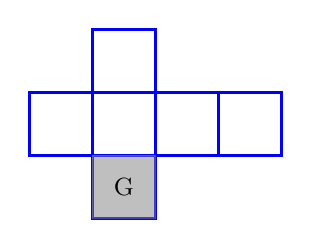
\begin{tikzpicture}[scale=0.8]
	% Würfelnetz in Kreuzform: vier Quadrate in einer Reihe, je eins oben und unten
	\foreach \x in {0,1,2,3}
		\draw[blue, very thick] (\x,0) rectangle ++(1,1);
	\draw[blue, very thick] (1,1) rectangle ++(1,1);
	\draw[blue, very thick] (1,-1) rectangle ++(1,1);
	% Grundfläche markieren
	\filldraw[gray, opacity=0.5] (1,-1) rectangle ++(1,1);
	\node at (1.5,-0.5) {\small G};
\end{tikzpicture}
\end{lstlisting}

\begin{ausgabe}
\centering
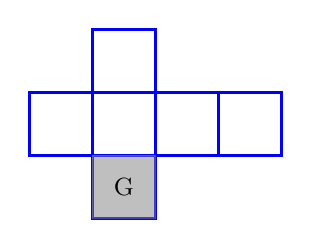
\begin{tikzpicture}[scale=0.8]
	% Würfelnetz in Kreuzform: vier Quadrate in einer Reihe, je eins oben und unten
	\foreach \x in {0,1,2,3}
		\draw[blue, very thick] (\x,0) rectangle ++(1,1);
	\draw[blue, very thick] (1,1) rectangle ++(1,1);
	\draw[blue, very thick] (1,-1) rectangle ++(1,1);
	% Grundfläche markieren
	\filldraw[gray, opacity=0.5] (1,-1) rectangle ++(1,1);
	\node at (1.5,-0.5) {\small G};
\end{tikzpicture}
\end{ausgabe}



%%%%  KAPITEL 6  %%%%
\section{Figuren auf dem Arbeitsblatt}

Eine Skizze steht neben den Teilaufgaben: \texttt{multicols}, links die Teilaufgaben, nach \texttt{\textbackslash columnbreak} die zentrierte \texttt{tikzpicture}:

\begin{lstlisting}[style=latex]
\begin{enumerate}[(1)]
	\item Gegeben ist das Dreieck $ABC$ mit $c = \unit[5]{cm}$ und $\alpha = 63^\circ$.
	\begin{multicols}{2}
		\begin{enumerate}[(a)]
			\item Konstruiere das Dreieck.
			\item Miss die Länge der Seite $a$.
			\item Berechne den Flächeninhalt.
		\end{enumerate}
		\columnbreak
		\centering
		\begin{tikzpicture}[scale=0.6]
			\coordinate (A) at (0,0);
			\coordinate (B) at (5,0);
			\coordinate (C) at (1.5,3);
			\pic[draw=red, thick, "$\alpha$", angle radius=0.6cm, angle eccentricity=1.6] {angle=B--A--C};
			\draw[blue, very thick] (A) -- (B) -- (C) -- cycle;
			\node[below left] at (A) {$A$};
			\node[below right] at (B) {$B$};
			\node[above] at (C) {$C$};
		\end{tikzpicture}
	\end{multicols}
\end{enumerate}
\end{lstlisting}

\begin{ausgabe}
\centering
\begin{enumerate}[(1)]
	\item Gegeben ist das Dreieck $ABC$ mit $c = \unit[5]{cm}$ und $\alpha = 63^\circ$.
	\begin{multicols}{2}
		\begin{enumerate}[(a)]
			\item Konstruiere das Dreieck.
			\item Miss die Länge der Seite $a$.
			\item Berechne den Flächeninhalt.
		\end{enumerate}
		\columnbreak
		\centering
		\begin{tikzpicture}[scale=0.6]
			\coordinate (A) at (0,0);
			\coordinate (B) at (5,0);
			\coordinate (C) at (1.5,3);
			\pic[draw=red, thick, "$\alpha$", angle radius=0.6cm, angle eccentricity=1.6] {angle=B--A--C};
			\draw[blue, very thick] (A) -- (B) -- (C) -- cycle;
			\node[below left] at (A) {$A$};
			\node[below right] at (B) {$B$};
			\node[above] at (C) {$C$};
		\end{tikzpicture}
	\end{multicols}
\end{enumerate}
\end{ausgabe}



%%%%  KAPITEL 7  %%%%
\section{Zusammenfassung}

Die wichtigsten Regeln:

\begin{itemize}
	\item Eckpunkte zuerst als \texttt{\textbackslash coordinate}, dann zeichnen
	\item Hauptfigur \texttt{blue, very thick}; Maße und Winkel \texttt{red, thick}; Konstruktion \texttt{gray, thin}; Flächen \texttt{gray, opacity=0.5}
	\item Winkel mit \texttt{\textbackslash pic\{angle=B--A--C\}}, rechte Winkel mit \texttt{right angle}
	\item Maßlinien \texttt{|<->|} mit Abstand zur Figur
	\item Körper in Kavalierperspektive ($45^\circ$, halbe Tiefe), verdeckte Kanten gestrichelt
	\item Skizze neben den Teilaufgaben mit \texttt{multicols} und \texttt{\textbackslash columnbreak}
\end{itemize}

Mit diesen Vorlagen lassen sich Geometrieaufgaben schnell und einheitlich gestalten.

\end{document}
